\documentclass{jpp}
\usepackage{graphicx}
\usepackage{caption}
\usepackage{listings}
\PassOptionsToPackage{hyphens}{url}\usepackage{hyperref}
%\usepackage{hyperref}
\usepackage{subcaption}
%\usepackage{hyperref} 
\usepackage{longtable}
% \usepackage{epstopdf, epsfig}

\hypersetup{
    colorlinks=true,
    linkcolor=blue,
    filecolor=magenta,      
    urlcolor=blue,
    pdfpagemode=FullScreen,
    breaklinks=true,
    }
    
\lstset{
  basicstyle=\ttfamily,
  columns=fullflexible,
  frame=single,
  breaklines=true,
  postbreak=\mbox{\textcolor{red}{$\hookrightarrow$}\space},
}

\usepackage[utf8]{inputenc}
\usepackage[T1]{fontenc}
\usepackage{amsmath}

\newtheorem{lemma}{Lemma}
\newtheorem{corollary}{Corollary}

\shorttitle{5291 Final Project}
\shortauthor{Group 16}

\title{Loan Origination Prediction
 Based on Various Machine Learning Models}

\author{Jiajia Song\aff{1} js5759,
  Yiyang Xu\aff{1} yx2612,
  Xuhao Meng\aff{1} xm2277,
  Yuchen Tang\aff{1} yt2754,
  Yucen Wang\aff{1} yw3561,
  Jia Qi Wang\aff{1} jw4001}

\affiliation{\aff{1}Department of Statistics, Columbia University}

\begin{document}

\maketitle

\section{Objective}

The mortgage loan has always been a controversial topic in the economy because it plays such an essential part in our whole economy. As we all know, the great recession during 2007 and 2008 was led by the collapse of subprime mortgages. There were defaults on high-risk housing loans, which caused the credit crunch in the global banking system (Field Ann). We can see that if large defaults take place, it would disturb the economy badly. To avoid a bad impact on the economy by not lending money to people who are likely to default, banks may change their loan origination behavior pattern. We are in urgent need of an up-to-date prediction model. Therefore, in this project, we try to come up with a model to predict if people get rejected in a mortgage loan request by using the individual data in New York from Consumer Financial Protection Bureau (CFPB). We choose the year 2017 data because 2017 can be regarded as the middle of an economic boom according to the federal funds rate (graph above). The FED ended open market operations in 2014 and started raising interest rates from the end of 2015 in order to decrease the money supply in the nation's financial systems. This encouraged banks to lend money less easily, which increased the lending rates and mortgage rates (Thangavelu). We can notice that mortgage rates went up over time from the end of 2015 according to the federal funds rate. It will be harder for people to get a mortgage than it was before 2016. Hopefully, the results from our project may provide insights into the up-to-date institution’s criterion. What’s more, we will relate them to the corresponding mortgage policies and provide a broader view of the loan origination. 

\section{Data Description}
\subsection{Variables}

Through implementing data validation and preprocessing on the raw dataset, we finally select nineteen variables to fit our models for further analysis. They may affect the loan origination process from different perspectives. For example, the income represents the applicants’ direct loan repayment ability. Some variables related to the house location may influence the potential appreciation. 

The description of the nineteen variables is listed in Table \ref{variables}.

\begin{center}
\begin{longtable}{|p{3cm}|p{10cm}|}
\caption{Variables Description} \label{variables} \\

\hline \multicolumn{1}{|l|}{\textbf{Variables}} &  \multicolumn{1}{l|}{\textbf{Descriptions}} \\ \hline 
\endfirsthead

\multicolumn{2}{c}%
{{\bfseries \tablename\ \thetable{} -- continued from previous page}} \\
\hline \multicolumn{1}{|l|}{\textbf{Variables}} & \multicolumn{1}{l|}{\textbf{Descriptions}} \\ \hline 
\endhead

\hline \multicolumn{2}{|r|}{{Continued on next page}} \\ \hline
\endfoot

\hline \hline
\endlastfoot


  \hline
  Agency & 1 -- Office of the Comptroller of the Currency (OCC) \\
         & 2 -- Federal Reserve System (FRS) \\ 
         & 3 -- Federal Deposit Insurance Corporation (FDIC) \\ 
         & 5 -- National Credit Union Administration (NCUA) \\ 
         & 7 -- Department of Housing and Urban Development (HUD) \\ & 9 -- Consumer Financial Protection Bureau (CFPB) \\
  \hline
  Loan Type  & 1 -- Conventional (any loan other than FHA, VA, FSA, RHS loans) \\ 
             & 2 -- FHA-insured (Federal Housing Administration) \\ 
             & 3 -- VA-guaranteed (Veterans Administration) \\ 
             & 4 -- FSA/RHS (Farm Service Agency or Rural Housing Service) \\
  \hline
  Property Type  & 1 -- One to four-family (other than manufactured housing) \\ 
  & 2 -- Manufactured housing \\ 
  & 3 -- Multifamily \\ 
  \hline
  Property Type  & 1 -- One to four-family (other than manufactured housing) \\ 
  & 2 -- Manufactured housing \\ 
  & 3 -- Multifamily \\ 
  \hline
  Loan Purpose & 1 -- Home purchase \\ 
  & 2 -- Home improvement \\ 
  & 3 -- Refinancing \\ 
  \hline
  Owner\_occupancy & 1 -- Owner-occupied as a principal dwelling \\
  & 2 -- Not owner-occupied \\ 
  & 3 -- Not applicable \\ 
  \hline
  Loan Amount & in thousands of dollars \\ 
  \hline
  Preapproval & 1 -- Pre Approval was requested \\ 
  & 2 -- Pre Approval was not requested \\ 
  & 3 -- Not applicable \\ 
  \hline
  Action\_taken  & 1 -- Loan originated \\ 
  & 2 -- Application approved but not accepted \\ 
  & 3 -- Application denied by financial institution \\ 
  \hline
  Applicant\_ethnicity & 1 -- Hispanic or Latino \\ 
  & 2 -- Not Hispanic or Latino \\ 
  & 3 -- Information not provided by applicant in mail, Internet, or telephone application \\ 
  & 4 -- Not applicable \\ 
  & 5 -- No co-applicant \\
  \hline
  Co-applicant Ethnicity & Same as above \\ 
  \hline
  Applicant Race & 1 -- American Indian or Alaska Native \\ 
  & 2 -- Asian \\ 
  & 3 -- Black or African American\\ 
  & 4 -- Native Hawaiian or Other Pacific Islander\\ 
  & 5 -- White\\ 
  & 6 -- Information not provided by applicant in mail, Internet, or telephone application\\ 
  & 7 -- Not applicable \\ 
  & 8 -- No co-applicant \\ 
  \hline
  Applicant Sex & 1 -- Male \\ 
  & 2 -- Female \\ 
  & 3 -- Information not provided by applicant in mail, Internet, or telephone application \\ 
  & 4 -- Not applicable \\ 
  &5 -- No co-applicant \\ 
  \hline
  Applicant Income & in thousands of dollars \\ 
  \hline
  Hud median family income & FFIEC Median family income in dollars for the\\ 
  & MSA/MD in which the tract is located (adjusted annually by FFIEC) \\ 
  \hline
  Tract to msamd income & \% of tract median family income\\ 
  & compared to MSA/MD median family income. (Carried to two decimal places) \\ 
  \hline
  Number of owner occupied units & Number of dwellings, including individual\\ 
  & condominiums that are lived in by the owner \\ 
  \hline
  Number of 1 to 4 family units & Dwellings that are built to house fewer than 5 families \\ 
  \hline
  Population & Total population in tract \\ 
  \hline
  Minority\_population & Percentage of minority population to total population for tract\\
  \hline
\end{longtable}
\end{center}

\subsection{EDA Parts}

We choose "action taken" as our response variable. The action\_taken equals 1 means the loan got approved. According to Figure \ref{EDA1}, through adding up the first two types of actions, nearly 79\% of loan applications got approved.

To have a deeper understanding of the relationships between our chosen predictors and the response variable, we generate multiple plots, which also shows the distributions of action taken in different values of independent variables. 

Figure \ref{EDA2} and Figure \ref{EDA3} show the visualization of the loan. ‘Home purchase’, ‘Home improvement’ and ‘Refinancing’ are indexed as 1, 2, and 3 respectively. Among the three existing loan purposes, ‘Home purchase’ is the most common one as over half of the mortgage applicants applied for loans for this reason. Meanwhile, it is interesting to see that the loan purpose called  ‘home improvement’ is least likely to get approved, as more applicants got rejected than accepted under this loan purpose. Besides, the density plot shows the loan amount distribution in 2017. The loan\_amount value follows the normal distribution and the median loan amount seems to be around \$200,000. 

Figure \ref{EDA4} shows the distribution of the six most frequent agency codes. It is quite clear that agencies called the Department of Housing and Urban Development(HUD) and Consumer Financial Protection Bureau (CFPB) got the most applicants. Comparatively, National Credit Union Administration (NCUA) has the highest approval rate among the six agencies.

The following four graphs show the distribution of different features of applicants’ information.  The loan approval and denial rate is falling under each category of the following four predictors.  Figure \ref{EDA5}, Figure \ref{EDA6}, and Figure \ref{EDA7} show detailed information related to the applicant's race, ethnicity, and sex. The number of male applicants is about 2 times higher than the number of female applicants. Figure \ref{EDA8} shows the density plot of applicant income. The distribution of applicant income also seems to be normally distributed, meanwhile, the median of applicant’s income is around \$100,000 according to the density plot.


\section{Data-preprocessing}

We preprocess our data from scratch, including handling NA’s and outliers, encoding the categorical variables, standardization, dealing with unbalanced data, and principal component analysis. 

Also, we divide the dataset into training and testing sets according to the ratio of 70-30. It is worth pointing out that due to a large amount of data and extremely slow speed of R, we sample 1,000 records out of all data for training and testing as a demo. 

\subsection{Cleaning and encoding}

\subsubsection{NA’s}

Many columns are mainly consisting of NA’s, which provides almost no information, so we drop such variables. After that, we drop the rows that contain NA’s, because the data volumes are so big, and we believe removing such rows would not change the distribution of our data. Detailed information of missing data can be viewed in Figure 9: Percentage of missing data by features.

\subsubsection{Outliers}

Some variables contain some extreme values, like the variables regarding incomes. They may affect the model training and even some of them are wrong data. We remove rows that are corresponding to the top 4\% quantile values. The threshold is arbitrary and the purpose is to remove some wrong records while keeping the distribution of the variables.

\subsubsection{Standardization}

Some models’ computations are based on distance, so if one of the features has a broad range of values, the distance will be affected by it and make this particular feature too important in the model. We use a z-score to standardize the numeric variables, which is like: 

$$x_{stand} = \frac{x-mean(x)}{sd(x)}$$

From Figure \ref{scale} , we can see that the data are scaled into the same range.

\begin{figure}
\begin{subfigure}{.5\textwidth}
  \centering
  % include first image
  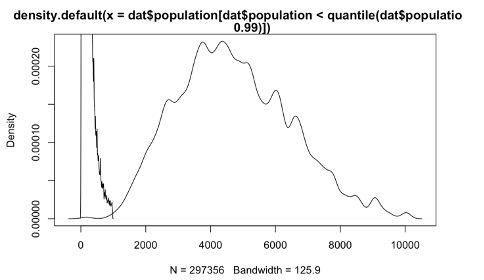
\includegraphics[width=.9\linewidth]{before_scale.png}  
  \caption{Before Standardization}
\end{subfigure}
\begin{subfigure}{.5\textwidth}
  \centering
  % include second image
  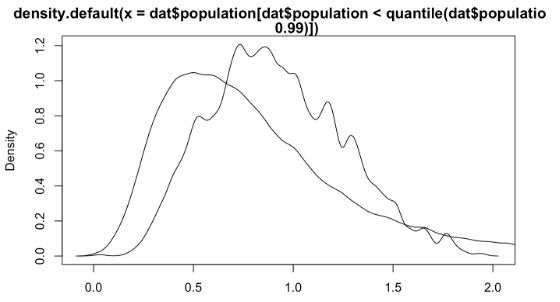
\includegraphics[width=.9\linewidth]{after_scale.png}  
  \caption{After Standardization}
\end{subfigure}
\caption{Standardization}
\label{scale}
\end{figure}


\subsubsection{Encoding/One-hot encoding}

Categorical variables can be represented by words, but numbers are better. Different classes are encoded by different numbers, and what’s more important is their `class()` in R. They should be `factor()` and never used as numbers in any models. Also, we use one-hot encoding to generate dummy variables corresponding to different classes. If the specific function in R can handle variables of class `factor()`, that is good. However, the one-hot encoding is a much more general method. 

\subsection{Unbalanced data: SmoteNC}

From the descriptive part above, we know that the data is unbalanced. There are many more people who get accepted than those who are rejected in loan requests. The unbalancedness may make the model not capture enough features of the minority class. Also, it would strongly influence the evaluation of the model prediction results. We use Synthetic Minority Over-sampling TEchnique-Nominal Continuous (SMOTE-NC) to handle this problem. It was created by Chawla, et.al. (2002). The algorithm is based on the Euclidean distance between the feature vectors for which k-nearest neighbors are being identified (minority class sample). The Figure \ref{smote} shows its basic concepts. 

\begin{figure}
  \centering
  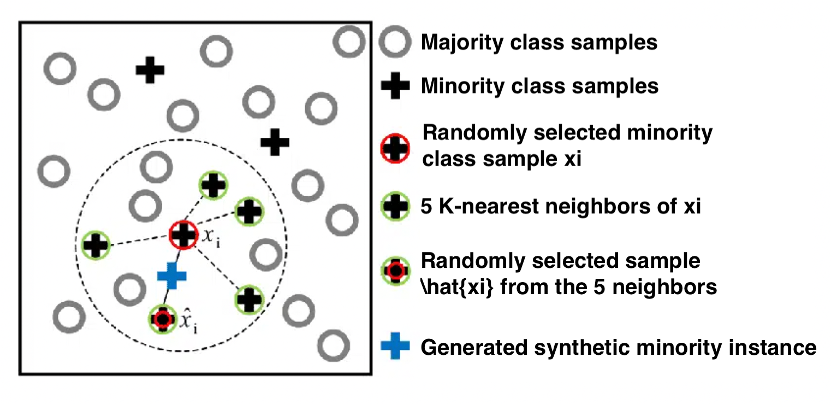
\includegraphics[width=.9\linewidth]{smote.png}
    \caption*{Source: \url{https://rikunert.com/smote\_explained}
    }
  \caption{SMOTE Algorithm}
  \label{smote}
\end{figure}

In our experiment, after SMOTE-NC, the labels of the dataset become balanced (536:536, previous 146:536). 

\subsection{Principal components for mixed data: FAMD}

Before creating the model, we check for multicollinearity. If there are high correlations between our variables, we need to deal with that problem. Variance Inflation Factor is a measure of multicollinearity for the variables, but it is usually applied to non-categorical variables. Since our model includes a mixture of categorical and non-categorical variables, we calculate the Generalized Variance Inflation Factor (GVIF) instead. GVIF is calculated as

$$GVIF = VIF^{\frac{1}{2*df}}$$

Our variables’ GVIF results are shwon in Figure \ref{gvif}.

\begin{figure}
  \centering
  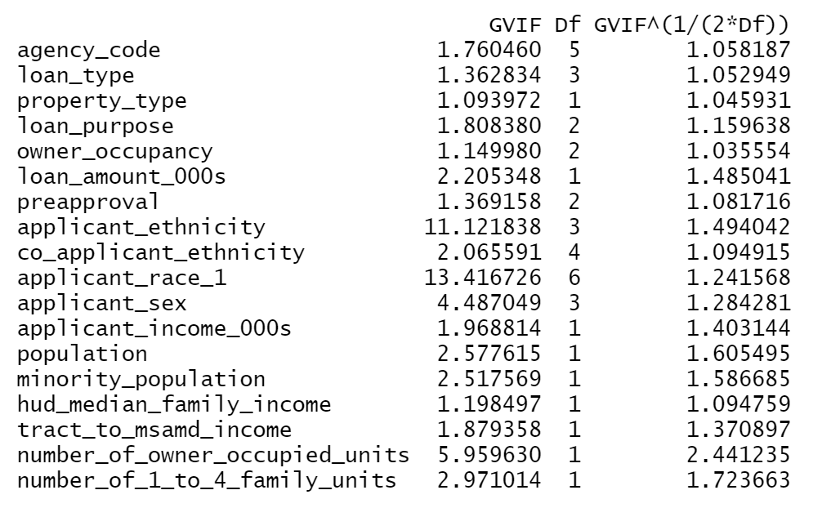
\includegraphics[width=.9\linewidth]{gvif.png}
  \caption{GVIF}\label{gvif}
\end{figure}

To check if there is a sign of multicollinearity, we compare the GVIF values with $10^{\frac{1}{2*df}}$. Thus, we find that applicant\_ethnicity and applicant\_race\_1 show a sign of multicollinearity.

In order to solve the multicollinearity problem and to filter out the variables with less important information, we consider the Principle Component Analysis method. We want to use the PCA algorithm to reduce dimensionality and extract the most important uncorrelated variables.

However, since our data includes both quantitative and qualitative variables, the normal PCA method is not applicable. We have to either use one-hot encoding to transform the categorical variables or use the Factorial Analysis of Mixed Data (FAMD) method. In fact, the one-hot encoding method does not work well. When we transform the categorical variables, one categorical variable will be changed to several variables depending on the number of the categories. Then, the results of PCA will not assign similar weights as the original variables. Therefore, we choose FAMD as a preprocessed method. FAMD applies the PCA algorithm on both quantitative and qualitative variables and assigns the same weights to variables.
 
We apply the "FAMD" function in R directly on our training data, and store the coordinates as our new estimates. The new model has eight dimensions, which can be used as preprocessed data for logistic regression, Random Forest model, and XGBoost model. The preprocessed data improves the logistic model, but not for Random Forest or XGBoost.

One problem for the FAMD preprocessed data is the loss of interpretation. Though the PCA method performs well in dealing with multicollinearity, it only solves the problem numerically. PCA rotates the data and creates new dimensions and our eighteen variables are shrunk to eight. Hence, it is difficult to interpret the variables for the new model.

Another problem is that the decision tree is immune to multicollinearity. Since Random Forest and XGBoost are based on decision trees, they are not affected by multicollinearity. Thus, using the FAMD method does not improve our model. Details will be shown in the Random Forest and XGBoost model section.

\section{Models}
\subsection{Logistic regression}

We first try to use logistic regression to fit the model. Logistic regression is a kind of predictive analysis that explains the relationship between one dependent variable and some independent variables. The reason why we choose logistic regression is that logistic regression can be used when the dependent variable (action\_taken) is binary and it can work out the probability of success of an event. To be specific, if the probability greater than 0.5 is classified as loan originated, otherwise, it is classified as loan denial. Moreover, logistic regression supports categorical data and about 55\% of our independent variables such as loan type and loan purpose can be converted to categorical variables. Finally, logistic regression is easy to implement and interpret. Therefore, it might be possible to work out an accurate model directly from logistic regression.

From Figure \ref{logistic}, we can see that the accuracy of the model is 65.67\%. However, the percentage of people who get a loan in the testing set is 80\%, which means the logistic regression model is much worse than a model that simply says everyone can get a loan.

\begin{figure}
\begin{subfigure}{.5\textwidth}
  \centering
  % include first image
  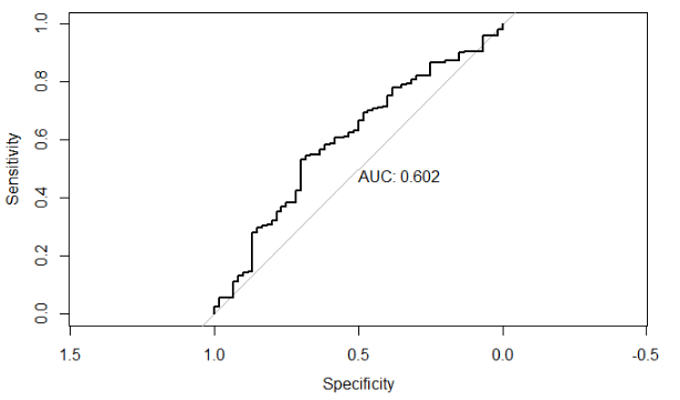
\includegraphics[width=.9\linewidth]{logistic1.png}  
  \caption{ROC Curve}
\end{subfigure}
\begin{subfigure}{.5\textwidth}
  \centering
  % include second image
  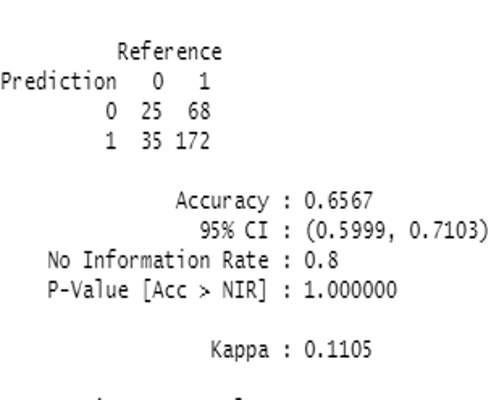
\includegraphics[width=.9\linewidth]{logistic2.png}  
  \caption{Confusion Matrix}
\end{subfigure}
\caption{Results for Logistic Regression}
\label{logistic}
\end{figure}

There are some reasons why logistic regression does not perform as well as we expected. 

The first reason might be the size of the dataset we used. A dataset of size 700 may not be large enough to include all cases of 19 variables. The second problem is that logistic regression assumes that the dependent variables and the independent variables have a linear relationship. However, variables such as applicant income and loan amount may not have a linear relationship with the probability of getting loans in reality. The third problem is that we might have ignored some interactions that affect the accuracy of prediction. 

We first try to investigate the interaction effect, and we are interested about interactions between agency name, loan type and loan purpose, as we think there must be some link between these three variables. 

For example, a person who wants to buy a house may have a higher chance of getting a loan when he applies for a loan insured by the Federal Housing Administration, and this may help us improve the accuracy of prediction.

And the way we evaluate the effectiveness of improvement of a single interaction is by calculating the accuracy of the model with that interaction and then comparing it to the accuracy of the model without any interactions.

As shown in Figure \ref{interaction}, adding interactions between any pairs of variables does not improve the accuracy of the model effectively. And when we added all three interactions into the model, the accuracy of the model is still 65\%. Therefore, we consider that adding interaction effects between variables does not significantly improve our model.

\begin{figure}
\begin{subfigure}{.475\textwidth}
  \centering
  % include first image
  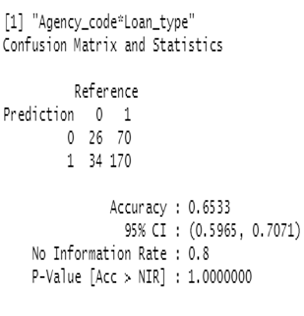
\includegraphics[width=.9\linewidth]{interaction1.png}  
  \caption{Interaction 1}
\end{subfigure}
\begin{subfigure}{.475\textwidth}
  \centering
  % include second image
  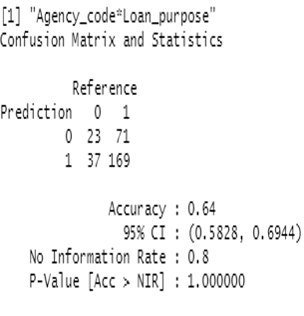
\includegraphics[width=.9\linewidth]{interaction2.png}  
  \caption{Interaction 2}
\end{subfigure}
\begin{subfigure}{.475\textwidth}
  \centering
  % include first image
  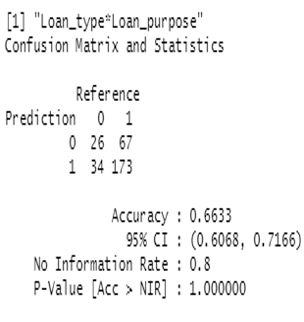
\includegraphics[width=.9\linewidth]{interaction3.png}  
  \caption{Interaction 3}
\end{subfigure}
\begin{subfigure}{.475\textwidth}
  \centering
  % include first image
  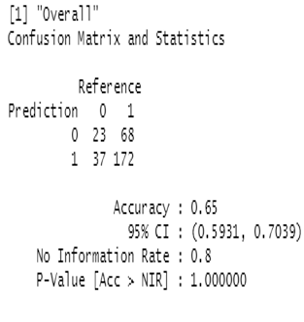
\includegraphics[width=.9\linewidth]{interaction4.png}  
  \caption{Interaction 4}
\end{subfigure}
\caption{Tests for Interactions}
\label{interaction}
\end{figure}

Finally, we fit the logistic regression model to our FAMD processed dataset. The result is shown in Figure \ref{logistic_FAMD}. The accuracy of the model is worsened from 65.67\% to 63.67\%, and it suggests that multicollinearity might not be a problem in our original dataset.

\begin{figure}
\begin{subfigure}{.5\textwidth}
  \centering
  % include first image
  \includegraphics[width=.9\linewidth]{logistic_FAMD1.png}  
  \caption{ROC Curve}
\end{subfigure}
\begin{subfigure}{.5\textwidth}
  \centering
  % include second image
  \includegraphics[width=.9\linewidth]{logistic_FAMD2.png}  
  \caption{Confusion Matrix}
\end{subfigure}
\caption{Results for Logistic regression Combined with FAMD}
\label{logistic_FAMD}
\end{figure}

\subsection{Artificial Neural network}

Among different types of neural networks, we choose the classic multilayer perceptron (MLP), which is based on a supervised procedure and consists of three layers: input, hidden, and output. It can handle both numeric variables and categorical variables by one-hot encoding. Also, we choose the resilient backpropagation learning algorithm, which is better than normal backpropagation. 

Due to the extremely slow speed in R, we are not able to try a lot of different network structures. Figure \ref{nn_structure} below shows the structure we tried. 

\begin{figure}
  \centering
  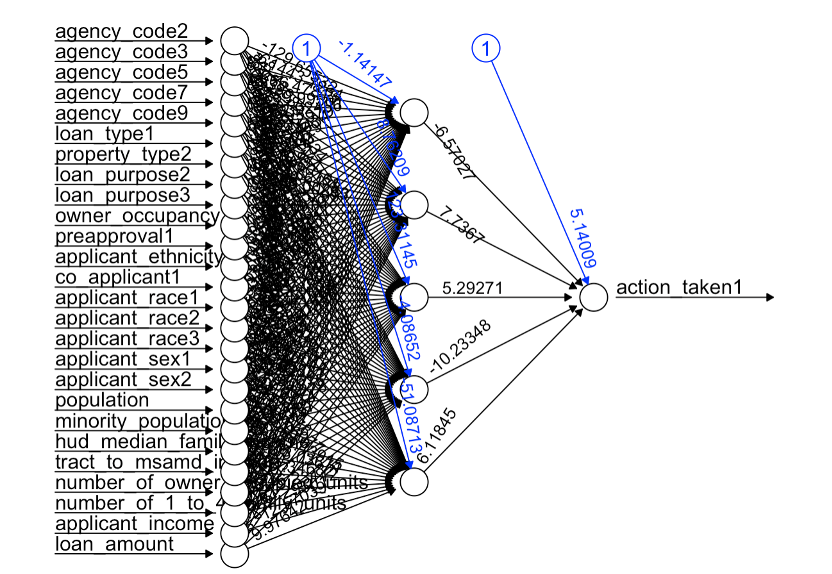
\includegraphics[width=.9\linewidth]{nn_structure.png}  
  \caption{Structure of Our ANN Model}
\label{nn_structure}
\end{figure}

Results are shown in Figure \ref{nn_results}, we can see that the model still can not capture the features why people get rejected and predict more True Negatives to be positive. As for the True positive samples, it performs well. 

\begin{figure}
  \centering
  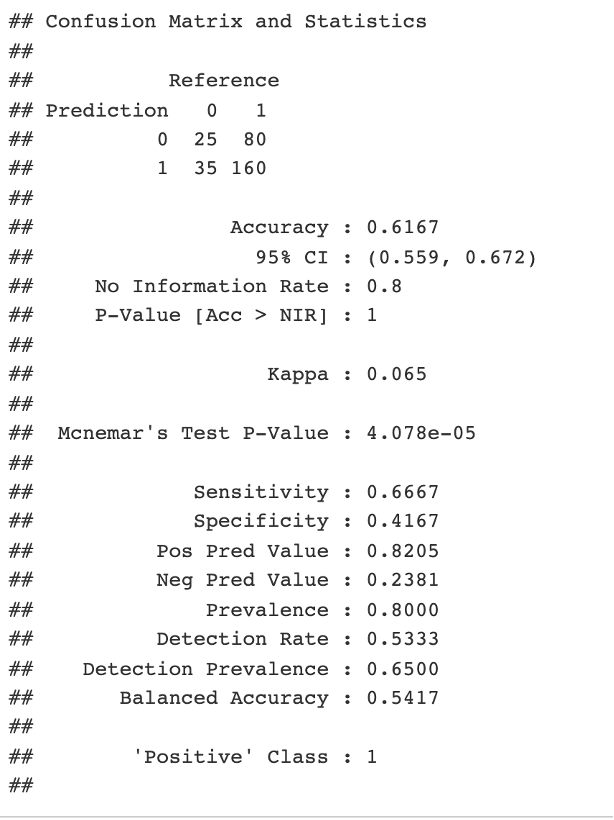
\includegraphics[width=.9\linewidth]{nn_results.png}  
  \caption{Structure of Our ANN Model}
\label{nn_results}
\end{figure}

Hyperparameters selection for neural networks and enough training time is of vital importance to a neural network. More complex or deep structures of neural networks should be tried systematically. After better hyperparameters selection, the performance of neural networks may improve. 

\subsection{Random forest}

The next attempt is using Random forest. Random forest is a type of machine learning technique that can be used for classification problems. It has some main advantages when working on our dataset. Firstly, it can work for both categorical and continuous variables. In our dataset, we have categorical variables like loan type and loan purpose, and we have continuous variables like applicant income and loan amount. Moreover, it works well with non-linear parameters. If applicant income does not have a linear relationship with the probability of getting a loan, the random forest will be a good choice dealing with this problem. Therefore, Random forest may be a better fit compared to logistic regression.

Then we start to fit a random forest. The function is shown in Figure \ref{rf_try}. One important parameter in the random forest is mtry, it is the number of variables randomly sampled as candidates at each split. We have 19 variables, so we can have mtry ranging from 1 to 19. And the accuracy of each fit is shown in Figure \ref{mtry_results}.

\begin{figure}
  \centering
  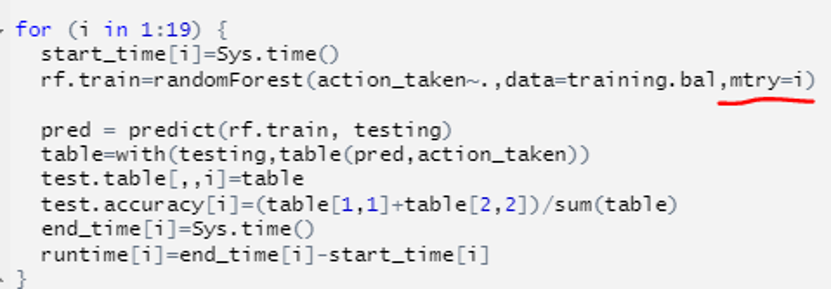
\includegraphics[width=.9\linewidth]{rf_try.png}  
  \caption{A Function to Test Different Hyperparameters for Random Forest}
\label{rf_try}
\end{figure}

\begin{figure}
  \centering
  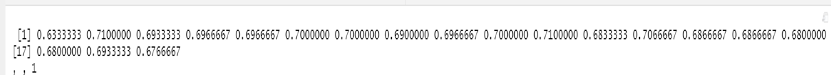
\includegraphics[width=.9\linewidth]{mtry_results.png}  
  \caption{Accuracy of Different mtry of Random Forest}
\label{mtry_results}
\end{figure}


We can see that mtry=2 is the optimal choice as the accuracy of prediction is the highest, and the accuracy of prediction is 71.00\%. It is more accurate compared to the logistic model. Although it is still worse than a model that simply says everyone can get a loan, we still consider this to be a good result as there is a huge improvement compared to the previous models.


\subsection{XGBoost}

After trying the tree model, we do not limit our scope of exploration as we try a new method called XGBoost, using decision trees as base learners. We hold the faith that this method might yield better results, as it is combining many weak learners to make a strong learner and is well-known as an ideal and efficient implementation of gradient boosting that can be used for classification predictive modeling. Meanwhile, XGBoost is a great fit for our dataset as it is well suited especially those related to real-world business problems such as fraud detection or customer churn prediction.

When we fit the XGBoost model, we use both training datasets that implemented SMOTE and FAMD balanced methods respectively. Randomness is used in the construction of the model. We also run cross-validation after each iteration. The result of the AUC and accuracy rate we get here is 0.612 and 0.7234  for the model using the SMOTE training datasets. Meanwhile, the AUC and accuracy rate we get for the FAMD balanced training dataset is 0.591 and 0.6632. It is obvious that the XGBoost model using the SMOTE regularization training dataset performs better than the XGBoost model using the FAMD balanced regularization. The XGBoost model using the SMOTE regularization also has a slightly higher AUC and accuracy rate than the random forest method. 

Figure \ref{xgboost_importance} selects significant predictors of the SMOTE regularized XGBoost model.

\begin{figure}
  \centering
  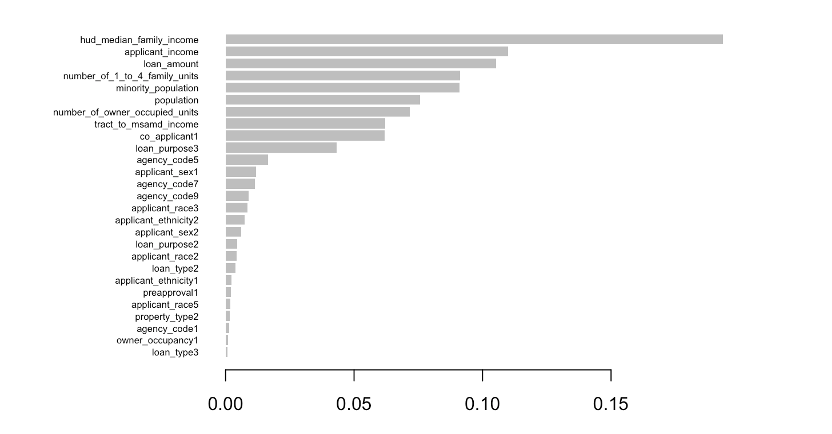
\includegraphics[width=.9\linewidth]{xgboost_importance.png}
  \caption{Importance of Variables in XGBoost}
\label{xgboost_importance}
\end{figure}

Although the XGBoost method is highly flexible, it still contains many shortcomings which may explain the unsatisfying result we got here. XGBoost does not perform well on sparse and unstructured data. Although we have already tried several methods to solve the highly sparse feature of our datasets, it may still cause much trouble when we try to apply the XGBoost method. 

For further expansion and improvement on this method, it is well-worth for us to keep trying and repeating the modeling process or performing systematic experimentation such as using a grid search across a range of values to find better hyperparameters. Meanwhile, when fitting a final model, it may be desirable to either increase the number of trees until the variance of the model is reduced across repeated evaluations, or to fit multiple final models and average their predictions.

\subsection{SVM}

From the previous data description section, we can see that all the independent variables in the data are labeled, which is loan denial or loan originated. This suggests that we can try to use SVM, which is a supervised learning model to classify two-type observations. There are potential benefits to using SVM, for example, it is very useful when data has a number of independent variables greater than the data size. Also, it can work efficiently in high-dimensional space. 

For SVM, We first find the points that lie closest to both the classes, which are support vectors. Then we try to find the proximity between our dividing plane and the support vectors. The distance between the points and the dividing line is called margin. What SVM is trying to do is to maximize the margin. When the margin is maximized, the hyperplane is what we are looking for. 

For the simple case, if we only have two features, the hyperplane will be 1 dimension, which is a line. (in Figure \ref{svm}) Because for this project, we have 10 features, we have a 9-dimensional subset that divides the space into two disconnected components.

\begin{figure}
  \centering
  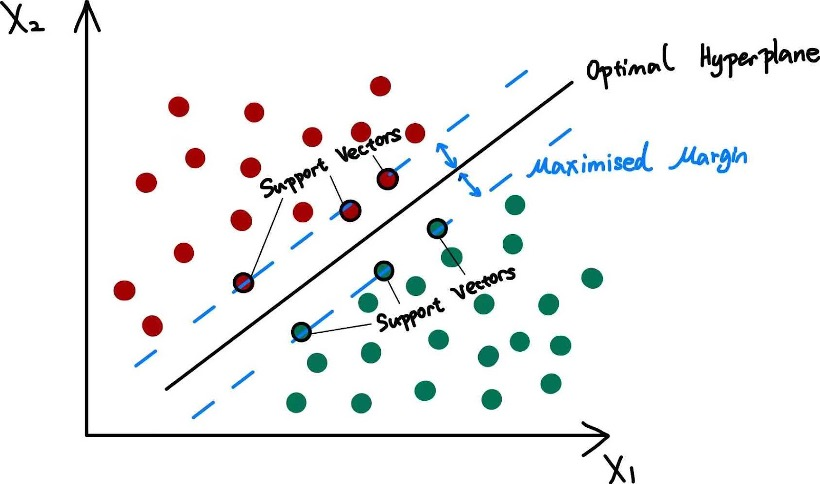
\includegraphics[width=.9\linewidth]{svm.jpg}  
  \caption{SVM Algorithm}
\label{svm}
\end{figure}

What we do in this project is to use a linear classifier by using a package "e1071" which contains the SVM function in R. Next we need to decide the cost argument in the SVM function because the cost quantifies the penalty to an observation on the wrong side of the classification boundary(misclassification). So we use the tune() function to test a sequence of costs and identify the value that gives the best fitting model. In this case, the cost = 0.1.(see Figure \ref{svm_costs})

\begin{figure}
  \centering
  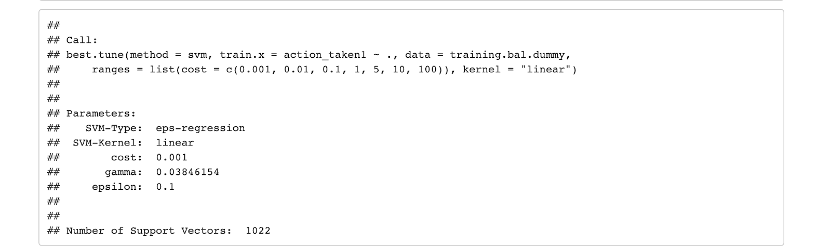
\includegraphics[width=.9\linewidth]{svm_cost.png} 
  \caption{SVM Cost Selection}
\label{svm_costs}
\end{figure}

Then, we try to come up with a model by setting cost = 0.1 in the SVM function. Then we use that model to predict the testing data, which is 30\% of our whole data. The SVM calculates the probability that a person gets approved, and we classify the probability greater than 0.5 as approval, otherwise, it is rejected. Then we get the confusion matrix, which is shown in Figure \ref{svm_results}. The error case is that the loan originated but the model classifies it as denial (False Positive) is about 8 times more than the case where the model misclassified the loan as originated but the loan is actually denied (False Negative). But we do not know the exact reason for this, which needs more future research. The accuracy of the model produced by SVM does not predict very well as the random forest model because the accuracy is only 50.33\%. Even though the data we are using here is balanced data, it does not help to improve this model. 

Besides, SVM has some disadvantages. When the data size is too large, the model is not expected to work well for a long training time. This is what we came across when we were doing this model,  we first tried the 5,000 data for the first time. But the SVM was too slow to generate the result. Then, we changed to trying 1,000 data, which SVM becomes much faster. This is the reason why the testing data is only 300.  

\begin{figure}
  \centering
  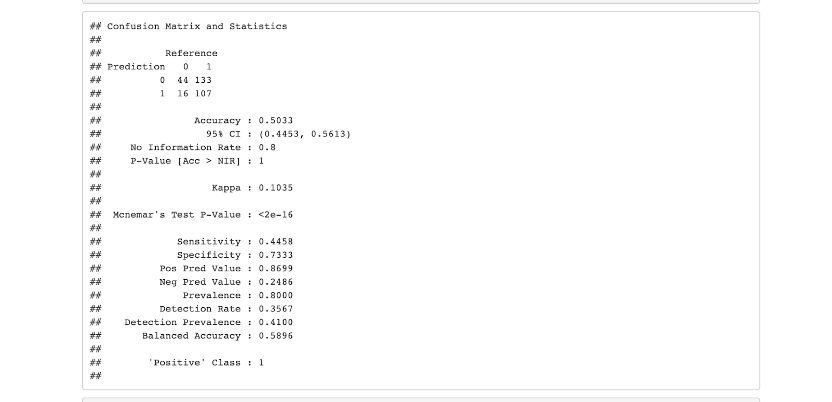
\includegraphics[width=.9\linewidth]{svm_results.png}  
  \caption{Results for SVM}
\label{svm_results}
\end{figure}


Besides, SVM has some disadvantages. When the data size is too large, the model is not expected to work well for a long training time. This is what we came across when we were doing this model,  we first tried the 5000 data for the first time. But the SVM is too slow to generate the result. Then, we changed to trying 1000 data, which SVM becomes much faster. This is the reason why the testing data is only 300.  

\section{Conclusions}

All in all,  the models we tried before do not perform very well. We have tried a lot of different measures to improve the model like rebalancing the data, but none of them shows significant improvements. However, from all our models, we can see there are some variables that always contribute a lot, like applicant income, loan amount, and loan purpose. It is reasonable to do the following research into loan origination.

\section{Problem and Limitations}

During the modeling of our dataset, we realize that there is another severe problem that holds us back from creating an accurate model, which is the lack of some key variables. For example, the dataset does not contain any information about peoples’ credit record, while credit record is one of the main factors that banks consider. Apart from credit records, variables such as employment status and bank savings are also missing from our dataset. The lack of key variables makes it hard to analyze banks’ behavior because they may behave differently while facing people of identical information. This would lead to misclassification while modeling the data and reduce the accuracy of our model. Those omitted variables in our data set will be fully discussed in the following section. We will dig into the problem in the next section. 

\section{Omitted variables}

Some regular criterias for applying for a mortgage successfully include a steady income and a dependable working history. It will be difficult for unemployed people to apply for a mortgage. A co-borrower can be a strategy to get a mortgage after unemployment since the loan lender will consider the co-borrower's income and his/her qualifications for the mortgage. Hence, a person who is employed or not may not be a big part of determining whether he/she can get the mortgage or not. 

Another variable might be the Loan-to-value ratio. According to the Consumer Financial Protection Bureau, the Loan to Value ratio needs to be taken into consideration as determining whether to lend the borrowers money or not. LTV is calculated as the amount of the loan compared to the appraised value of the property (LTV Ratio). Higher LTV ratios for borrowers show higher risks to lenders. For our data, we have a "loan\_amount" variable but need the "value of the property" to calculate the LTV ratio. The Department of the Treasury also emphasizes the importance of the appraised value of the mortgage, "While borrowers’ ability to repay their real estate loans according to reasonable terms remains the primary consideration in the lending decision, an institution also must consider the value of the underlying real estate collateral in accordance with the Agencies’ appraisal regulations" (Department of the Treasury, page 8). It issued Interagency Appraisal and Evaluation Guidelines, providing appraisal standards for evaluations and examiners. Some basic examination contents include the location of the property, current and projected use of the property, estimated market value in the actual physical condition, and property-specific data (Department of the Treasury, page 13). However, these are not the only factors that influence the appraised value. The evaluation methods vary depending on different agencies and the validity may change due to the time and market conditions. Therefore, we need more data to calculate the LTV ratio to improve our model.

In addition, an article on the Time points out several standards that mortgage underwriting is looking at like credit history, Debt-to-income ratio, income verification, and so on (Lauren). For our project, the data set does not have information about the credit history of an individual. As mentioned in the article, those are very important to determine if a person’s mortgage loan gets approved. 

Other essential factors are included in the FICO score. Wells Fargo provides the constitution of FICO scores, ranging from 300 to 850. The higher the FICO score, the less risky the borrowers (Wells Fargo). Table \ref{fico} shows factors that affect FICO scores. Due to the lack of data, the model might generate some errors when predicting. 

\begin{center}
\begin{longtable}{|l|l|}
\caption{Factors for FICO Score} \label{fico} \\

\hline \multicolumn{1}{|l|}{\textbf{FICO Score Factors}} &  \multicolumn{1}{l|}{\textbf{Descriptions}} \\ \hline 
\endfirsthead

\multicolumn{2}{c}%
{{\bfseries \tablename\ \thetable{} -- continued from previous page}} \\
\hline \multicolumn{1}{|l|}{\textbf{FICO Score Factors}} & \multicolumn{1}{l|}{\textbf{Descriptions}} \\ \hline 
\endhead

\hline \multicolumn{2}{|r|}{{Continued on next page}} \\ \hline
\endfoot

\hline \hline
\endlastfoot


  \hline
  Payment History (35\%) & Payments on time \\
         & Frequency of missed payments \\ 
         & Passed due dates \\ 
         & Recent missed payments \\ 
         & Payments 30 days past due\\ 
         & Number of accounts (showing late payment)\\
  \hline
  Money Owed (30\%) & Entire amount owed \\
         & Number and types of accounts \\ 
         & Proportion of money owed compared to credit available \\ 
  \hline
         Length of credit history (15\%) & Average age of credit \\
  \hline
  Types of accounts (10\%) & Mix of accounts \\
         & Installment loans \\ 
         & Home loans \\ 
         & Retail and credit cards \\ 
  \hline
  Recent credit activity (10\%) & Recently opened accounts \\
         & Other high risky actions \\ 
  \hline
\end{longtable}
\end{center}


\clearpage


\section{References}

Berry, Craig. "Can You Buy a House or Get a Mortgage on Unemployment?" Mortgage Rates, Mortgage News and Strategy: The Mortgage Reports, 6 Aug. 2021, \url{https://themortgagereports.com/70823/buy-a-house-on-unemployment-income}.

Chawla, N. V., Bowyer, K. W., Hall, L. O., \& Kegelmeyer, W. P. (2002). SMOTE: synthetic minority over-sampling technique. Journal of artificial intelligence research, 16, 321-357.

Department of the Treasury. "Interagency Appraisal and Evaluation Guidelines". Journal Register, vol. 75, no. 237, 10 Dec. 2010, \url{https://www.govinfo.gov/content/pkg/FR-2010-12-10/pdf/2010-30913.pdf}. Accessed 5 Dec. 2021. 

LTV Ratio, "What Is a Loan-to-Value Ratio and How Does It Relate to My Costs?", Consumer Financial Protection Bureau, 9 Sept. 2020, \url{https://www.consumerfinance.gov/ask-cfpb/what-is-a-loan-to-value-ratio-and-how-does-it-relate-to-my-costs-en-121}. 

Pupale, Rushikesh. "Support Vector Machines(Svm) - an Overview." Towards Data Science, 11 Feb. 2019, \url{https://towardsdatascience.com/https-medium-com-pupalerushikesh-svm-f4b42800e989}.

Thangavelu, Poonkulali. "How the Federal Reserve Affects Mortgage Rates?" Investopedia, Investopedia, 3 Dec. 2021, \url{https://www.investopedia.com/articles/personal-finance/050715/how-federal-reserve-affects-mortgage-rates.asp}. 

Wells Fargo, "How Your Credit Score Is Calculated." Wells Fargo, \url{https://www.wellsfargo.com/financial-education/credit-management/calculate-credit-score/}.

Ward, Lauren. "What Is Mortgage Underwriting? Explaining The Underwriting Process." Time, Time, 24 Aug. 2021, \url{https://time.com/nextadvisor/mortgages/underwriting-process}.

\appendix

\section{Exploratory Data Analysis (EDA)}\label{EDA}

\begin{figure}
\begin{subfigure}{.5\textwidth}
  \centering
  % include first image
  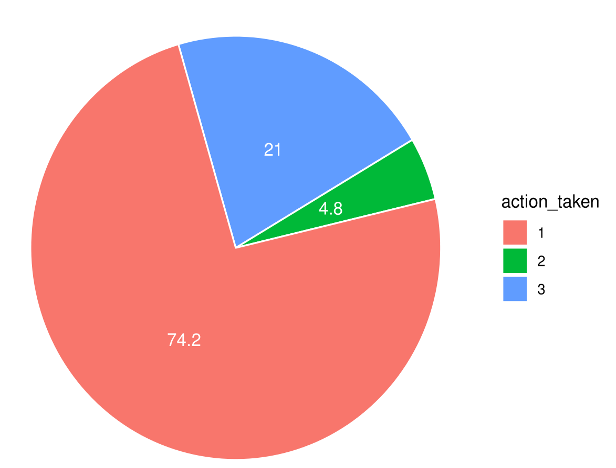
\includegraphics[width=.9\linewidth]{EDA1.png}  
  \caption{Visualization of dependent variable}\label{EDA1}
\end{subfigure}
\begin{subfigure}{.5\textwidth}
  \centering
  % include second image
  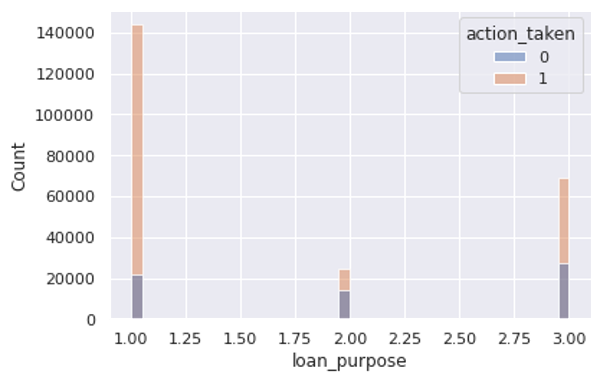
\includegraphics[width=.9\linewidth]{EDA2.png}  
  \caption{Visualization of loan}\label{EDA2}
\end{subfigure}
\begin{subfigure}{.5\textwidth}
  \centering
  % include first image
  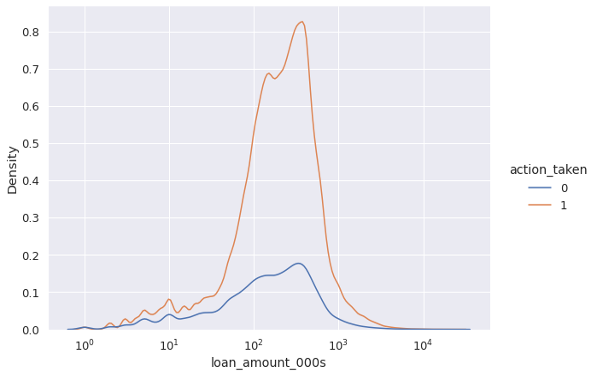
\includegraphics[width=.9\linewidth]{EDA3.png}  
  \caption{Density plot of loan }\label{EDA3}
\end{subfigure}
\begin{subfigure}{.5\textwidth}
  \centering
  % include first image
  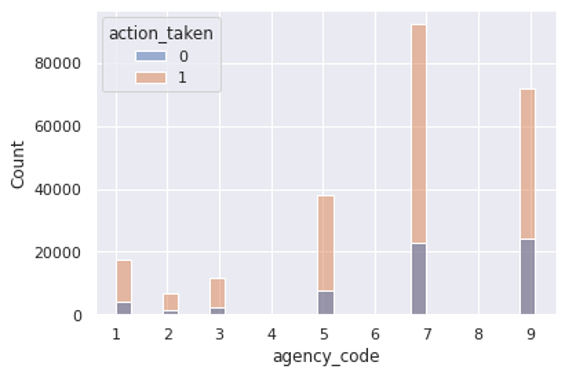
\includegraphics[width=.9\linewidth]{EDA4.png}  
  \caption{Visualization of agency code}\label{EDA4}
\end{subfigure}
\begin{subfigure}{.5\textwidth}
  \centering
  % include first image
  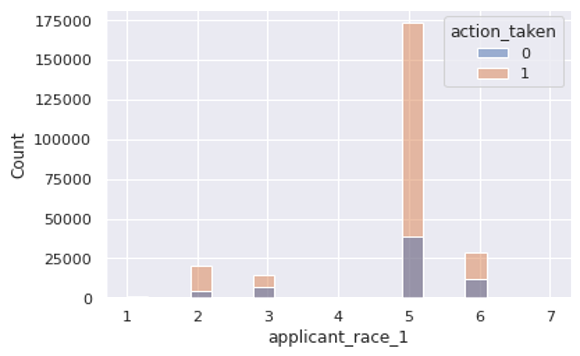
\includegraphics[width=.9\linewidth]{EDA5.png}  
  \caption{Visualization of applicant race}\label{EDA5}
\end{subfigure}
\begin{subfigure}{.5\textwidth}
  \centering
  % include first image
  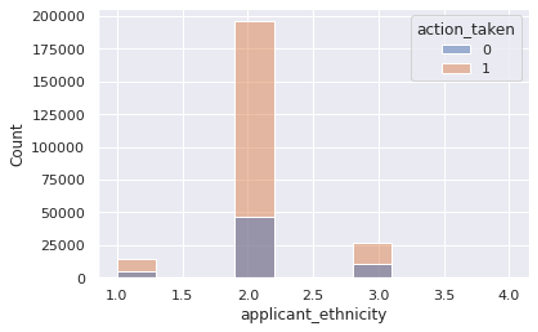
\includegraphics[width=.9\linewidth]{EDA6.png}  
  \caption{Visualization of applicant ethinicity}\label{EDA6}
\end{subfigure}
\begin{subfigure}{.5\textwidth}
  \centering
  % include first image
  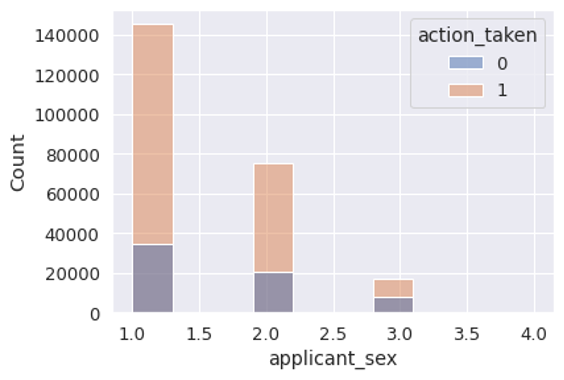
\includegraphics[width=.9\linewidth]{EDA7.png}  
  \caption{Visualization of applicant sex}\label{EDA7}
\end{subfigure}
\begin{subfigure}{.5\textwidth}
  \centering
  % include first image
  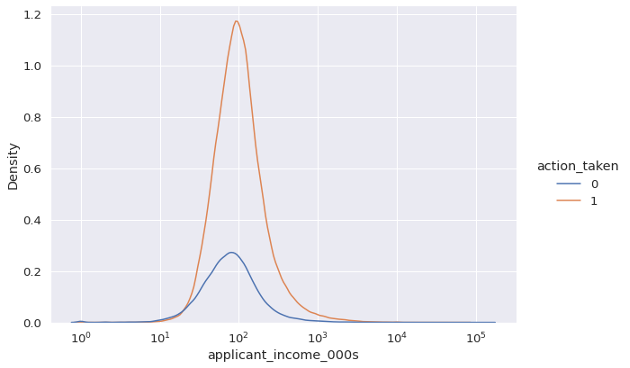
\includegraphics[width=.9\linewidth]{EDA8.png}  
  \caption{Density plot of applicant income}\label{EDA8}
\end{subfigure}
\caption{Exploratory Data Analysis (EDA): Part 1}
\label{EDA}
\end{figure}

\begin{figure}
  \centering
  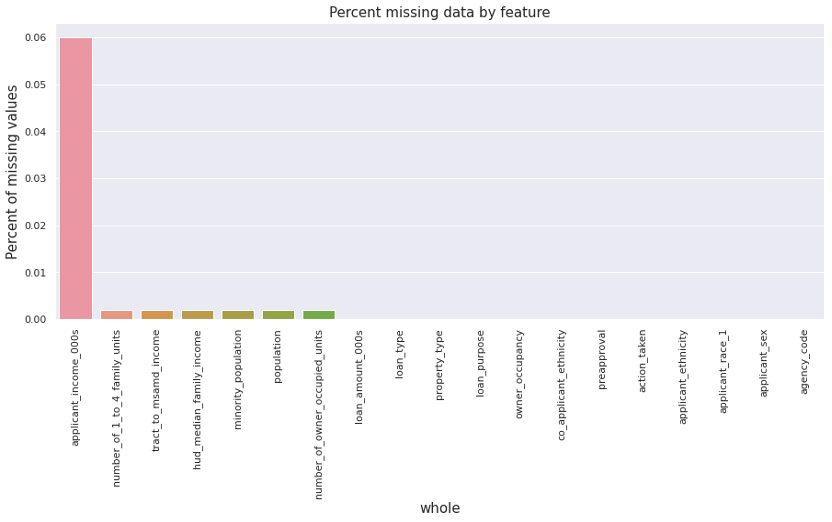
\includegraphics[width=.9\linewidth]{EDA9.png}  
  \caption{Exploratory Data Analysis (EDA): Part 2: Percentage of missing data by features}\label{EDA9}
\end{figure}

\clearpage
\section{R Code}\label{code}
\begin{lstlisting}[language=R]
library(tidyverse)
library(glmnet)
library(caret)
library(pROC)

dat <- read.csv("/Users/yctang/Documents/Columbia/5291 Advanced data Analysis/project/data/hmda_2017_ny_all-records_labels.csv")
# remove some variables & NA
dat <- subset(dat, select = -c(1:4, 6, 8, 10, 12, 15, 17, 19:27, 29, 31, 33:50, 51, 53, 54, 56:71, 69:71, 78))

## Data Pre-processing
# drop missing values
dat <- drop_na(dat)

# some adjustments: re-encoding
# owner_occupancy: other == 0, Owner-occupied as a principal dwelling == 1
dat[dat$owner_occupancy == 2, ]$owner_occupancy <- 0
dat[dat$owner_occupancy == 3, ]$owner_occupancy <- 0
# loan_type: other == 0, Conventional == 1
dat[dat$loan_type == 2, ]$loan_type <- 0
dat[dat$loan_type == 3, ]$loan_type <- 0
dat[dat$loan_type == 4, ]$loan_type <- 0
# preapproval: not requested == 0
dat[dat$preapproval == 2, ]$preapproval <- 0
dat[dat$preapproval == 3, ]$preapproval <- 0
# action_taken
dat = dat %>% filter(action_taken == 1 | action_taken == 2 | action_taken == 3)
dat[dat$action_taken == 2, ]$action_taken <- 1
dat[dat$action_taken == 3, ]$action_taken <- 0
# applicant_ethnicity: other == 0, hispanic/latino == 1
dat[dat$applicant_ethnicity == 2, ]$applicant_ethnicity <- 0
dat[dat$applicant_ethnicity == 3, ]$applicant_ethnicity <- 0
dat[dat$applicant_ethnicity == 4, ]$applicant_ethnicity <- 0
# sex: unknown == 0, male == 1, female == 2
dat[dat$applicant_sex == 3, ]$applicant_sex <- 0
dat[dat$applicant_sex == 4, ]$applicant_sex <- 0
# race: other == 0, asian == 1, Black or African American == 2, white == 3
dat[dat$applicant_race_1 == 1, ]$applicant_race_1 <- 0
dat[dat$applicant_race_1 == 4, ]$applicant_race_1 <- 0
dat[dat$applicant_race_1 == 6, ]$applicant_race_1 <- 0
dat[dat$applicant_race_1 == 7, ]$applicant_race_1 <- 0
dat[dat$applicant_race_1 == 2, ]$applicant_race_1 <- 1
dat[dat$applicant_race_1 == 3, ]$applicant_race_1 <- 2
dat[dat$applicant_race_1 == 5, ]$applicant_race_1 <- 3
names(dat)[names(dat) == "applicant_race_1"] <- "applicant_race"
# co-applicant, yes/no == 1/0
dat[dat$co_applicant_ethnicity == 2, ]$co_applicant_ethnicity <- 1
dat[dat$co_applicant_ethnicity == 3, ]$co_applicant_ethnicity <- 0
dat[dat$co_applicant_ethnicity == 4, ]$co_applicant_ethnicity <- 0
dat[dat$co_applicant_ethnicity == 5, ]$co_applicant_ethnicity <- 0
names(dat)[names(dat) == "co_applicant_ethnicity"] <- "co_applicant"

# Change classes of variables
dat$agency_code <- as.factor(dat$agency_code)
dat$loan_type <- as.factor(dat$loan_type)
dat$property_type <- as.factor(dat$property_type)
dat$loan_purpose <- as.factor(dat$loan_purpose)
dat$owner_occupancy <- as.factor(dat$owner_occupancy)
dat$preapproval <- as.factor(dat$preapproval)
dat$action_taken <- as.factor(dat$action_taken)
dat$applicant_ethnicity <- as.factor(dat$applicant_ethnicity)
dat$co_applicant <- as.factor(dat$co_applicant)
dat$applicant_race <- as.factor(dat$applicant_race)
dat$applicant_sex <- as.factor(dat$applicant_sex)

## Data Visualization

dat %>%
  ggplot(aes(action_taken, fill = action_taken)) + 
  geom_bar()+
  scale_y_continuous(labels = scales::percent)

## Training-testing Set Split

set.seed(123456)
indices.old <- sample(1:nrow(dat), nrow(dat) * 0.7)
training.old <- dat[indices.old, ]
testing.old <- dat[-indices.old, ]

## First Try: Logistic Regression

full <- glm(action_taken ~., family = binomial(link = 'logit'), data = training.old)
#summary(fit)
test.prob <- predict(full, testing.old, type = "response")
test.pred <- as.numeric(ifelse(test.prob > 0.5, 1, 0))
confusionMatrix(data = as.factor(test.pred), reference = testing.old$action_taken, positive = "1")
test.roc <- roc(testing.old$action_taken ~ test.prob, plot = TRUE, print.auc = TRUE)

## Outliers, standardization and other adjustments

# outliers & standardization
hist(dat$applicant_income_000s)
plot(density(dat$population[dat$population < quantile(dat$population, 0.99)]))
lines(density(dat$applicant_income_000s[dat$applicant_income_000s < quantile(dat$applicant_income_000s, 0.99)]))

dat <- dat %>%
  filter(applicant_income_000s < quantile(applicant_income_000s, 0.96)) %>%
  filter(loan_amount_000s < quantile(loan_amount_000s, 0.96)) %>%
  mutate(applicant_income = as.numeric(scale(applicant_income_000s, center = FALSE)), 
         loan_amount = as.numeric(scale(loan_amount_000s, center = FALSE)), 
         population = as.numeric(scale(population, center = FALSE)), 
         hud_median_family_income = as.numeric(scale(hud_median_family_income, center = FALSE)),
         number_of_owner_occupied_units = as.numeric(scale(number_of_owner_occupied_units, center = FALSE)),
         number_of_1_to_4_family_units = as.numeric(scale(number_of_1_to_4_family_units, center = FALSE)),
         minority_population = minority_population / 100,
         tract_to_msamd_income = tract_to_msamd_income / 100
         ) %>%
  dplyr::select(-c(applicant_income_000s, loan_amount_000s)) %>%
  dplyr::select(action_taken, everything())

hist(dat$applicant_income)
plot(density(dat$population))
lines(density(dat$applicant_income))
plot(density(dat$population[dat$population<quantile(dat$population, 0.99)]))
lines(density(dat$applicant_income[dat$applicant_income<quantile(dat$applicant_income, 0.99)]))

## Second Try: Logistic Regression

set.seed(123456)
dat <- sample_n(dat, 1000)
indices <- sample(1:nrow(dat), nrow(dat) * 0.7)
training <- dat[indices, ]
testing <- dat[-indices, ]
full <- glm(action_taken ~., family = binomial(link = 'logit'), data = training)
#summary(fit)
test.prob <- predict(full, testing, type = "response")
test.pred <- as.numeric(ifelse(test.prob > 0.5, 1, 0))
confusionMatrix(data = as.factor(test.pred), reference = testing$action_taken, positive = "1")
test.roc <- roc(testing$action_taken ~ test.prob, plot = TRUE, print.auc = TRUE)

## SMOTE & L1 Regularization

# install the RSBID package
#install.packages("devtools")
#devtools::install_github("dongyuanwu/RSBID")
library(RSBID)
#training.dummy$action_taken1 <- as.factor(training.dummy$action_taken1)
#testing.dummy$action_taken1 <- as.factor(testing.dummy$action_taken1)

ptm <- proc.time()
training.bal <- SMOTE_NC(training, "action_taken")
proc.time() - ptm # running time

training.bal.dummy <- data.frame(model.matrix( ~ ., training.bal)[, -1])
testing.dummy <- data.frame(model.matrix( ~ ., testing)[, -1])
X <- as.matrix(training.bal.dummy[-1])
Y <- training.bal.dummy$action_taken1
cv <- cv.glmnet(X, Y, family = "binomial")
fit.L1 <- glmnet(X, Y, family = "binomial", alpha = 1, lambda = cv$lambda.min)
# confusion matrix and roc curve
test.prob <- fit.L1 %>% predict(newx = as.matrix(testing.dummy[-1]))
test.pred <- as.numeric(ifelse(test.prob > 0.5, 1, 0))
mean(test.pred == testing.dummy$action_taken1)
confusionMatrix(data = as.factor(test.pred), reference = factor(testing.dummy$action_taken1), positive = "1")
test.roc <- roc(testing.dummy$action_taken1 ~ as.numeric(test.prob), plot = TRUE, print.auc = TRUE)

## Logistic interaction

fit=glm(action_taken~.,family = "binomial",data=training.bal)

# confusion matrix and roc curve
test.prob <-  predict(fit, testing, type = "response")
test.pred <- as.numeric(ifelse(test.prob > 0.5, 1, 0))
mean(test.pred == testing$action_taken)
confusionMatrix(data = as.factor(test.pred), reference = factor(testing$action_taken), positive = "1")
test.roc <- roc(testing$action_taken ~ as.numeric(test.prob), plot = TRUE, print.auc = TRUE)

## interaction

fit=glm(action_taken~.+agency_code*loan_type,family = "binomial",data=training.bal)

# confusion matrix and roc curve
test.prob <-  predict(fit, testing, type = "response")
test.pred <- as.numeric(ifelse(test.prob > 0.5, 1, 0))
print("Agency_code*Loan_type")
confusionMatrix(data = as.factor(test.pred), reference = factor(testing$action_taken), positive = "1")
test.roc <- roc(testing$action_taken ~ as.numeric(test.prob), plot = TRUE, print.auc = TRUE)

fit=glm(action_taken~.+agency_code*loan_purpose,family = "binomial",data=training.bal)

# confusion matrix and roc curve
test.prob <-  predict(fit, testing, type = "response")
test.pred <- as.numeric(ifelse(test.prob > 0.5, 1, 0))
print("Agency_code*Loan_purpose")
confusionMatrix(data = as.factor(test.pred), reference = factor(testing$action_taken), positive = "1")
test.roc <- roc(testing$action_taken ~ as.numeric(test.prob), plot = TRUE, print.auc = TRUE)

fit=glm(action_taken~.+loan_type*loan_purpose,family = "binomial",data=training.bal)
# confusion matrix and roc curve
test.prob <-  predict(fit, testing, type = "response")
test.pred <- as.numeric(ifelse(test.prob > 0.5, 1, 0))
print("Loan_type*Loan_purpose")
confusionMatrix(data = as.factor(test.pred), reference = factor(testing$action_taken), positive = "1")
test.roc <- roc(testing$action_taken ~ as.numeric(test.prob), plot = TRUE, print.auc = TRUE)

#Overall

fit=glm(action_taken~.+agency_code*loan_type+agency_code*loan_purpose+loan_type*loan_purpose,family = "binomial",data=training.bal)

# confusion matrix and roc curve
test.prob <-  predict(fit, testing, type = "response")
test.pred <- as.numeric(ifelse(test.prob > 0.5, 1, 0))
print("Overall")
print("Overall")
confusionMatrix(data = as.factor(test.pred), reference = factor(testing$action_taken), positive = "1")
test.roc <- roc(testing$action_taken ~ as.numeric(test.prob), plot = TRUE, print.auc = TRUE)

full <- glm(action_taken~., family = binomial(link = "logit"), data = training.bal.FAMD)
test.prob <- predict(full, testing.bal.FAMD, type = "response")
test.pred <- as.numeric(ifelse(test.prob > 0.5, 1, 0))
confusionMatrix(data = as.factor(test.pred), reference = testing$action_taken, positive = "1")
test.roc <- roc(testing$action_taken ~ test.prob, plot = TRUE, print.auc = TRUE)

## Try: Neural Network

library(neuralnet)
ptm <- proc.time()
set.seed(123456)
NN = neuralnet(action_taken1 ~ ., training.bal.dummy, hidden = 5, linear.output = FALSE, err.fct = 'ce', stepmax = 1e7)
proc.time() - ptm # running time
plot(NN)
predict_NN = compute(NN, testing.dummy[-1])
test.pred <- as.numeric(ifelse(predict_NN$net.result > 0.5, 1, 0))
mean(test.pred == testing.dummy$action_taken1)
confusionMatrix(data = as.factor(test.pred), reference = factor(testing.dummy$action_taken1), positive = "1")
test.roc <- roc(testing.dummy$action_taken1 ~ predict_NN$net.result, plot = TRUE, print.auc = TRUE)

## FAMD

library(FactoMineR)
library(factoextra)
options(ggrepel.max.overlaps = Inf)

# unbalanced
FAMD1 <- FAMD(training[, -1], ncp = 8)
training.FAMD <- data.frame(FAMD1$ind$coord)
training.FAMD$action_taken <- training$action_taken
testing.FAMD <- data.frame(predict.FAMD(FAMD1, testing[, -1])$coord)
testing.FAMD$action_taken <- testing$action_taken
#balanced
FAMD2 <- FAMD(training.bal[, -1], ncp = 8)
training.bal.FAMD <- data.frame(FAMD2$ind$coord)
training.bal.FAMD$action_taken <- training.bal$action_taken
testing.bal.FAMD <- data.frame(predict.FAMD(FAMD2, testing[, -1])$coord)
testing.bal.FAMD$action_taken <- testing$action_taken

# FAMD unbalanced training set
full <- glm(action_taken ~ ., family = binomial(link = "logit"), data = training.FAMD)
test.prob <- predict(full, testing.FAMD, type = "response")
test.pred <- as.numeric(ifelse(test.prob > 0.5, 1, 0))
confusionMatrix(data = as.factor(test.pred), reference = testing$action_taken, positive = "1")
test.roc <- roc(testing$action_taken ~ test.prob, plot = TRUE, print.auc = TRUE)

# FAMD balanced training set
full <- glm(action_taken ~ ., family = binomial(link = "logit"), data = training.bal.FAMD)
test.prob <- predict(full, testing.bal.FAMD, type = "response")
test.pred <- as.numeric(ifelse(test.prob > 0.5, 1, 0))
confusionMatrix(data = as.factor(test.pred), reference = testing$action_taken, positive = "1")
test.roc <- roc(testing$action_taken ~ test.prob, plot = TRUE, print.auc = TRUE)

### Randomforest mtry1-19

library(randomForest)
test.accuracy = double(19)
test.table=array(0,c(2,2,19))
runtime=double(19)
start_time=rep(NA,19)
end_time=rep(NA,19)

for (i in 1:19) {
  start_time[i]=Sys.time()
  rf.train=randomForest(action_taken~.,data=training.bal,mtry=i)

  pred = predict(rf.train, testing)
  table=with(testing,table(pred,action_taken))
  test.table[,,i]=table
  test.accuracy[i]=(table[1,1]+table[2,2])/sum(table)
  end_time[i]=Sys.time()
  runtime[i]=end_time[i]-start_time[i]
}

test.accuracy
test.table

## Random Forest

library(randomForest)
# class of label/dependent variables should be `factor` -> classification
#training.bal.dummy$action_taken1 <- as.factor(training.bal.dummy$action_taken1)
rf_model <- randomForest(action_taken ~ ., data = training.bal, proximity = TRUE)
print(rf_model)
# type = "prob" -> gets the probability
rf_prob <- predict(rf_model, testing, type = "prob")[, 2]

#calculate RMSE
#sqrt(mean((rf_pred - testing.dummy$action_taken1)^2))

test.pred.rf <- as.numeric(ifelse(rf_prob > 0.5, 1, 0))
confusionMatrix(data = as.factor(test.pred.rf), reference = testing$action_taken, positive = "1")
test.rf.roc <- roc(testing$action_taken ~ rf_prob, plot = TRUE, print.auc = TRUE)

# ROC for training set
#rf.roc <- roc(training.bal$action_taken, rf_model$votes[, 2], plot = TRUE, print.auc = TRUE)

# RandomForest based on FAMD balanced data
rf_model2 <- randomForest(action_taken ~ ., data = training.bal.FAMD, proximity = TRUE)
print(rf_model2)
rf_prob <- predict(rf_model2, testing.bal.FAMD, type = "prob")[, 2]

test.pred.rf <- as.numeric(ifelse(rf_prob > 0.5, 1, 0))
confusionMatrix(data = as.factor(test.pred.rf), reference = testing$action_taken, positive = "1")
test.rf.roc <- roc(testing$action_taken ~ rf_prob, plot = TRUE, print.auc = TRUE)

### XGBOOST

library(xgboost)
testing_label <- testing[, 1] #define testing label(copy from below lines)
training_sparse <- sparse.model.matrix(action_taken ~ . - 1, training.bal)
training_label <- training.bal[, 1]
train_matrix <- xgb.DMatrix(data = training_sparse, label = as.numeric(training_label) - 1)
testing_sparse <- sparse.model.matrix(action_taken ~ . - 1, testing)
test_matrix <- xgb.DMatrix(data = testing_sparse, label = as.numeric(testing_label) - 1)

params <- list(booster = "gbtree", objective = "binary:logistic", eta = 0.3, gamma = 0, max_depth = 6, min_child_weight = 1, subsample = 1, colsample_bytree = 1)
xgb.cv <- xgb.cv(params = params, data = train_matrix, nfold = 5, nrounds = 100)
##best iteration =

xgb1 <- xgb.train(params = params, data = train_matrix, nrounds = 100, watchlist = list(val = test_matrix, train=train_matrix), print_every_n = 10, early_stop_round = 10, maximize = F , eval_metric = "error")

xgb.prob <- predict(xgb1, test_matrix)
xgb.pred <- ifelse (xgb.prob > 0.5, 1, 0)
confusionMatrix(data = as.factor(xgb.pred), reference = testing_label, positive = "1")
test.rf.roc <- roc(testing$action_taken ~ xgb.prob, plot = TRUE, print.auc = TRUE)

mat1 <- xgb.importance(feature_names = colnames(training_sparse), model = xgb1)
xgb.plot.importance(importance_matrix = mat1)

# xgboost based on FAMD balanced training data

training_sparse <- sparse.model.matrix(action_taken ~ . - 1, training.bal.FAMD)
training_label <- training.bal[, 1]
train_matrix <- xgb.DMatrix(data = training_sparse, label = as.numeric(training_label) - 1)
testing_sparse <- sparse.model.matrix(action_taken ~ . - 1, testing.bal.FAMD)
testing_label <- testing[, 1]
test_matrix <- xgb.DMatrix(data = testing_sparse, label = as.numeric(testing_label) - 1)

params <- list(booster = "gbtree", objective = "binary:logistic", eta = 0.3, gamma = 0, max_depth = 6, min_child_weight = 1, subsample = 1, colsample_bytree = 1)
xgb.cv <- xgb.cv(params = params, data = train_matrix, nfold = 5, nrounds = 100)
##best iteration =

xgb2 <- xgb.train(params = params, data = train_matrix, nrounds = 100, watchlist = list(val = test_matrix, train=train_matrix), print_every_n = 10, early_stop_round = 10, maximize = F , eval_metric = "error")

xgb.prob <- predict(xgb2, test_matrix)
xgb.pred <- ifelse(xgb.prob > 0.5, 1, 0)
confusionMatrix(data = as.factor(xgb.pred), reference = testing_label, positive = "1")
test.rf.roc <- roc(testing$action_taken ~ xgb.prob, plot = TRUE, print.auc = TRUE)

mat2 <- xgb.importance(feature_names = colnames(training_sparse), model = xgb2)
xgb.plot.importance(importance_matrix = mat2)

### SVM

library(e1071)
tune.out <- e1071::tune(svm,action_taken1 ~ ., data = training.bal.dummy, kernel = "linear", ranges = list(cost = c(0.001, 0.01, 0.1, 1, 5, 10, 100)))
# extract the best model
(bestmod <- tune.out$best.model)

svmfit = e1071::svm(action_taken1 ~ ., data = training.bal.dummy, kernel = "linear", cost = 0.001, scale = FALSE)

probs <- predict(svmfit, testing.dummy)
preds <- as.numeric(ifelse(probs > 0.5, 1, 0))

confusionMatrix(data = as.factor(preds), reference = as.factor(testing.dummy$action_taken1), positive = "1")

test.roc <- roc(testing.dummy$action_taken1 ~ probs, plot = TRUE, print.auc = TRUE)
\end{lstlisting}

\end{document}
